\documentclass[14pt,fleqn]{extarticle}
\RequirePackage{prepwell}

\previewoff 

\begin{document} 
\begin{snippet}
    
    \incorrect
    
    The area under the curve $y = \sqrt{x-1}$ between $x=1$ and $x=5$ is as shown below 
    
    \begin{center}

\includegraphics[scale=1.4]{wrong.eps}
\end{center}
    
    \reason
    
    $y = \sqrt{x-1} \implies y^2 = x - 1$. This looks like a parabola \newline 
    
    Bit notice also that $ y =0$ when $x = 1$. Hence, if anything, the parabola 
    should look like this 
    
    \begin{center}
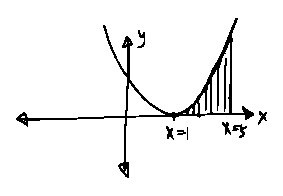
\includegraphics[scale=1.4]{right.eps}
\end{center}

    And the required area is the shaded bit 
    
\end{snippet} 
\end{document} 